\documentclass[10pt, a4paper]{report}

\usepackage[]{graphicx}
\usepackage[]{hyperref}
\usepackage{listings}
\usepackage{color}
\usepackage{parskip}
\definecolor{codegreen}{rgb}{0,0.6,0}
\definecolor{codegray}{rgb}{0.5,0.5,0.5}
\definecolor{codepurple}{rgb}{0.58,0,0.82}
\definecolor{backcolour}{rgb}{0.95,0.95,0.92}
 
\lstdefinestyle{mystyle}{
    backgroundcolor=\color{backcolour},   
    commentstyle=\color{codegreen},
    keywordstyle=\color{magenta},
    numberstyle=\tiny\color{codegray},
    stringstyle=\color{codepurple},
    basicstyle=\footnotesize,
    breakatwhitespace=false,         
    breaklines=true,                 
    captionpos=b,                    
    keepspaces=true,                 
    numbers=left,                    
    numbersep=5pt,                  
    showspaces=false,                
    showstringspaces=false,
    showtabs=false,                  
    tabsize=2
}
 
\lstset{style=mystyle,language = C++}
\usepackage[utf8]{inputenc}

%\lstset{
% 	frame = single,
% 	language = C++,
% 	showstringspaces = false,
% 	tabsize = 2,
% 	otherkeywords = {self},
% 	keywordstyle = \color{blue},
% 	identifierstyle=\color{deepgreen},
% 	stringstyle=\color{orange},
% 	backgroundcolor=\color{mygray}
%}

\title{Diffusion Transport in nanoporous SiO$_2$ \\
  \hrulefill\small{ Fys2880 }\hrulefill}
  
\author{Joseph Knutson \\
\href{https://github.com/mathhat/}{\texttt{github.com/mathhat}}}
  
\begin{document}

\begin{titlepage}
\maketitle
\begin{abstract}

\end{abstract}

\tableofcontents
\end{titlepage}
\chapter{Introduction}
\section*{sdgsg}


\chapter{Theory}

\section*{Molecular Dynamics (MD)}
Molecular Dynamics is a computer simulation method for estimating the motion of atoms and molecules.
The method creates N-body simulations that show how dynamic systems of particles evolve over time. To dictate how the particles move, we apply interatomic potentials. These potentials
simulate energies and forces that puts our system in motion. By mathematically integrating Newton's equations of motion,
we can find properties such as velocity, local temperatures and diffusion. The catch of solving N-body problems through MD integration is that errors will accumulate over time.
To minimize errors, one has to choose the proper algorithm and parameters for the system.

\section*{The MD Program}
A Molecular Dynamics program begins with initiating a state, then simulating it over time through mathematical means.
This section is a simple overview of how an MD program is set up.

\subsection*{Initiating a state}
In order to begin an MD program, you first need an initial state:
\begin{itemize}
 \item {\bf{Initial Positioning}}
 
Particles are initially placed in either ordered or random positions.
Another way to initiate the particles' positions is to load a previous state from an earlier simulation.
We're going to use all three methods.
\item {\bf{Initial Velocity}}

In our case, the particles' initial velocities follow a random (gaussian) distribution related to the initial temperature of the system.
\item {\bf{Potential}}
In order to make our particles act realistically, we apply an interatomic potential. 
This potential dictates how the particles behave. A potential creates forces between the particles, 
making them attracted to each other, or the opposite.
Potentials between different particles usually spawns different behaviour. 
Hydrogen atoms will for example interact differently with oxygen than silicat.
\end{itemize}
\subsection*{Bringing the System to Life}
After creating an initial state, you want movement. The initial velocity and the interatomic 
potential will from here on decide where our particles will travel. In order to simulate the particles' paths,
we need to integrate Newton's equations of motion over a time step. A time step is a small interval of time in 
which our system goes from its present state to a new one. 

Imagine an apple falling from a tree. Initially, it is connected to a tree branch, its velocity equals zero.
Gravity then does its work.
A second later, the apple is disconnected from the branch. The apple now has a new position and a new velocity.
Another second passes and the apple is closer to the ground, while the velocity keeps increasing.

This is an example of an MD program where the particle is an apple. 
When the apple was connected to the tree branch phase, the system was in its initial state. 
The gravity acted as the potential and the seconds as time steps. In order to foresee where the apple 
would be a second in the future, one would simply need the apple's present position, velocity and the gravitational force, 
relative to the Earth.

From the falling apple example, we understand that position and velocity, as well as gravity is essential for knowing where 
the apple would end up in the next time step.

Here is a technical formula for bringing a system to life:
\begin{itemize}
 \item {\bf{Gather Present Properties}}
Gather information such as the position and velocity of the particles.
Calculate the forces working on each particle by looking at positioning and potential.
 \item {\bf{Use Present Properties to Simulate Future State}}
 
Possessing the present forces at work, we can numerically integrate these forces over a time step 
(fragment of a second).
When we do this, we're given the particles' positions and velocities a step forward in time.
 \item {\bf{Repeat}}

 New positions, means new forces. These forces can again be integrated and give birth to more changes in position and velocity.
 The amount of repetitions, or \emph{runs}, usually depends on your problem. In our apple example, if your timestep is as big as 
 a second and your goal is for the apple to reach the ground, you would only need 5 runs, 5 seconds.
 The simulation time will depend on the amount of runs, the size of your system and your computational power.
 
 Bear in mind that for each run you simulate, more error will accumulate.

\item {\bf{Sample}}

After your program has finished running, dump/sample the data for later simulations and analysis.
\end{itemize}

\section*{Structure of Code}
I have chosen to use LAMMPS as my code language.
LAMMPS is a classical molecular dynamics code, and an acronym for Large-scale Atomic/Molecular Massively Parallel Simulator.\footnote{http://lammps.sandia.gov/}
This section aims to give you a basic intuition of how LAMMPS algorithms are written.
For a random simulation, the structure of a program file will typically look like this:

\begin{lstlisting}[language=C++]
# ----------------- Init Section -----------------

include "system.init" 
//Initializes units and simulation box


# ----------------- Atom Definition Section -----------------

read_data "system.data"  
//Loads presaved state

# ----------------- Settings Section -----------------

include "system.settings" 
//Defines particles and potentials between them


# ----------------- Run Section -----------------

run   5000 			
//Integrates over 5000 time steps

write_data filename.data	
//Sample/save the resulting state
\end{lstlisting}
The first line of code includes a file called ``\emph{system.init}''. Including is merely adding all the code written inside the file you include.
Inside this file
lies the code that defines what units were using. SI units are not often practical since we're dealing with relatively small values.
The initialization process also defines the volume and shape of the system. Our simulations will be done inside a box.

The second line of code has a command called ``read\textunderscore data''.
This command looks for a data file, typically containing information about a state from a previous simulation.
Sometimes the data file contains much less than a system of particles, e.g. a single water molecule. The molecule can then be multiplied
and viola, you have a system of water.

The third line of code includes a file called ``\emph{system.settings}''.
After having loaded a state of particles, they have already been assigned types.
This part of the program tells particles how to interact with each other and how much each individual particle type is supposed to weigh.
The last part of setting up your system is usually assigning a temperature.

The last lines of code brings the system in motion. The line orders the system to move one time step towards the future, 5000 times.
The ``write\textunderscore data'' command, saves the final state inside a datafile. 


\chapter{The Problem}
We want try to determine wether or not water's self diffusion will change as a result of changes to the shape of its nanoporous surroundings.
Liquid water, as any other fluid, experiences internal motion. Inside the fluid, the water molecules are wobbling and crashing together, causing
transportation. This transportation of particles is called self diffusion. Water's self diffusion depends on many things, such as pressure, temperature and boundary conditions.

We want to inspect if the self diffusion of water behaves differently
when encapsuled in different geometries of SiO$_2$ nanopores. This is plausible due to water being polar and interacts therefore with polar materials such as silicat. 
Because water inside silicat nanopores is so tightly encapsulated, the electromagnetic interactions between the water 
molecules and the silicat might cause noticeable changes to the water's self diffusion.
This chapter will further discuss the nature of our hypothesis and how we aim to test it.

\section{Diffusion}
Diffusion is described as the netto movement of fluidic particles. A high diffusion coefficient translates to a lot of random motion in your system.
In order to measure the self diffusion of our water we have applied two methods: MSD, the \emph{mean squared displacement} method and VACF, the \emph{velocity autocorrelation function} method.
These methods will be discussed further under the ``Methods'' chapter.

As stated earlier, diffusion is a function of both temperature and pressure. Overall, high temperature causes both transport of particles and violent fluctuations.
Transportation and vibrations are then taken into account when measuring the diffusion of the system. Also local pressure changes set particles in motion.

The potential is useful to take into account while discussing the diffusion of a fluid. The potential of a substance decides/describes the substance attributes. These could be attributes such as viscosity, polarity, etc.
Polarity is something we find in water, where there is a local imbalance of the electromagnetic field. This causes water to stick to certain materials, e.g. glass surfaces. The point of this project is to see if
the potential conjures up forces that makes water behave differently than normal under new circumstances. The circumstances being that the water is inside of nanoporous silicat.

\section{Nanopores and Silicat}
We will simulate 2 types of nanopores. Spherical and cylindrical. I don't think nanopores tend not to look like perfect spheres, 
but the idea is to see if there is a diffusion change based on the shape of the nanopore.
It is within these pores that the water will reside.
Not only will we compare the diffusion of water within different shapes of pores, we will also change the volume of the pores in order to find additional diffusional patterns.

Glass, crystall, quarts and many other materials are solids made up of silicat networks.
The silicat network we initiatially work with is called beta cristobalite or $\beta$-cristobalite, see figure \ref{fig:beta}.
\begin{figure}[h] 

 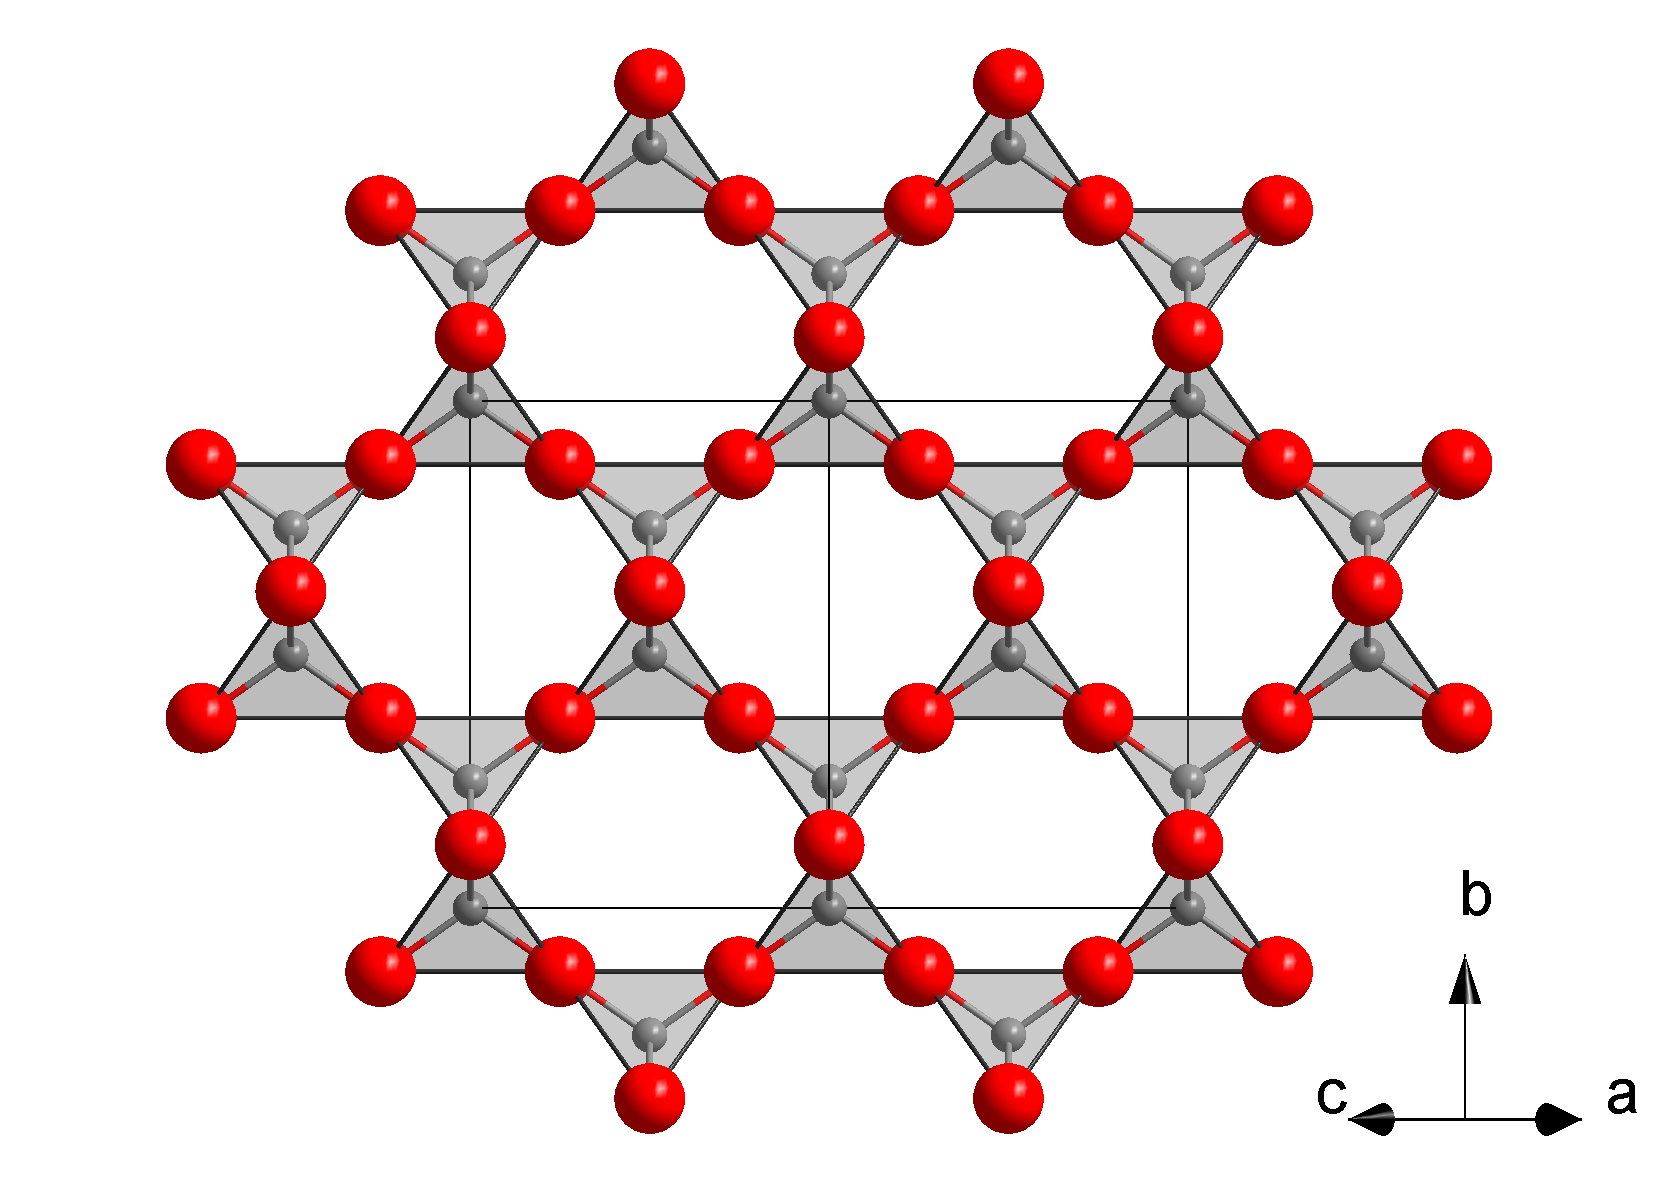
\includegraphics[scale=0.15]{beta.png}\centering
 \caption{\label{fig:beta}Silicat in the form of $\beta$-cristobalite. Each silicon atom (white) is connected to 4 oxygen atoms (red).}
 
\end{figure}
Figure \ref{fig:beta} does not satisfy our criteria for a simulated


The reason why I emphasize that this is our initial silicate network is because we are going to melt it.
We want an amorphous and chaotic structure that resembles the silicat inside the Earth's crust and we can only get this by melting the crystal structure.
After melting the crystal, we quickly cool it so that the structure remains amorphous.




\begin{figure}[h] 

 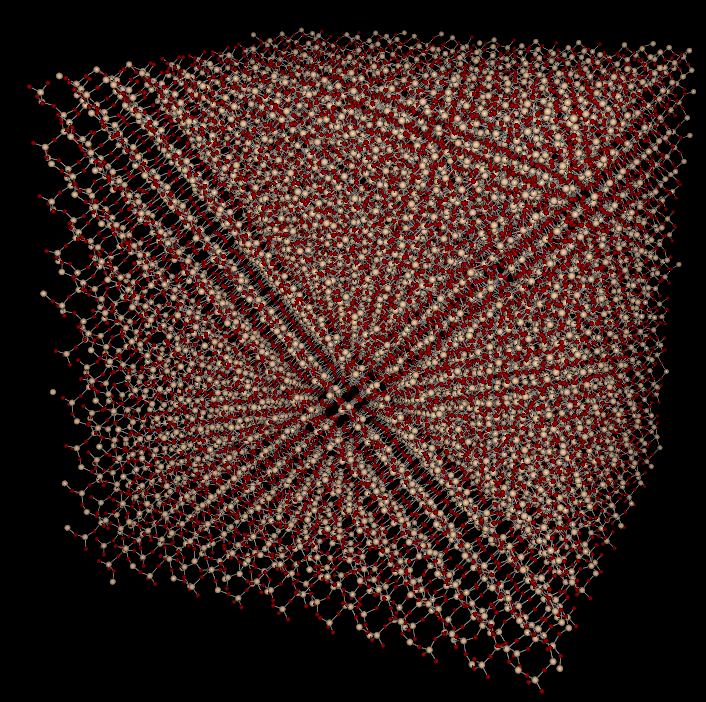
\includegraphics[scale=0.35]{block}\centering
 \caption{\label{fig:pores}Block of $\beta$-cristobalite. Written in lammps, .}
 
\end{figure}


To look at water inside of SiO$_2$ chambers, we first need to create the chambers.



\chapter{Methods}

This chapter discusses our general methods of Molecular Dynamics in further detail and the other methods relevant to the problem.


\begin{thebibliography}{9}

\bibitem{morten2}
	Hiorth-Jensen, M.,
	\emph{Project 2, Computational Physics I FYS3150/FYS4150},
	University of Oslo,
	2016.
	
\bibitem{abel}
	Abel, N.H.,
	Memoire sur le équations algébriques, ou l'on démontre l'impossibilité de la résolution de l'équation générale de cinquiéme degré,
	In Sylow, L. and Lie, S., 
	\emph{Æuvres Complètes de Niels Henrik Abel}, 2nd ed.,
	Grøndahl \& Søn, pp. 28-33,
	1881.

\end{thebibliography}

\begin{appendix}
\section{Laguerre Polynomials}
\label{app:laguerre}
Generally, the name Laguerre polynomials is used for solutions to 
\begin{equation}
x\frac{d^2y}{dx^2}+(\alpha+1-x)\frac{dy}{dx} + ny = 0.
\end{equation}
These polynomials, usually denoted, $L_0$, $L_1$, $L_2$ etc are a polynomial sequence which may be defined by the Rodriguez formula
\begin{equation}
L_n(x) = \frac{e^x}{n!}\frac{d^n}{dx^n}(e^{-x}x^n)=\frac{1}{n!}\left(\frac{d}{dx} -1 \right)x^n
\end{equation}
The first few Laguerre polynomials are shown in table \ref{tab:laguerre}.

\begin{table}[ht]
	\centering
	\caption{The first few Laguerre polynomials}
	\begin{tabular}{cl} \hline
	$n$ & $L_n(x)$  \\ \hline
	$0$ & $1$ \\
	$1$ & $-x+1$ \\
	$2$ & $\frac{1}{2}(x^2-4x+2)$ \\
	$3$ & $\frac{1}{6}(-x^3+9x^2-18x+6)$ \\
	$4$ & $\frac{1}{24}(x^4-16x^3+72x^2-96x+24$ \\
	$5$ & $\frac{1}{120}(-x^5+25x^4-200x^3+600x^2-600x+120) $ \\
	$6$ & $\frac{1}{720}(x^6-36x^5+450x^4-2400x^3+5400x^2-4320x+720)$ \\ \hline
	\end{tabular}
	\label{tab:laguerre}
\end{table}

\end{appendix}

\end{document}